\documentclass{article}


\graphicspath{{/home/david/Book/Chapters/2.Vectors/DotProduct/pic/}}
% !TeX root = ../../../Mainfile/book.tex



\begin{document}

\color{white}
\subsection{Vector dot product}
\color{black}

\begin{equation*}
 \icol{\color{rooj} 1 \\ \color{groen} 3 \color{black} } \bullet \icol{\color{rooj} 4 \\ \color{groen} 1 \color{black} } = \color{rooj} 1 \cdot 4  \color{black} + \color{groen}  3 \cdot 1 \color{black} = 7
\end{equation*}





\paragraph{Dot product:} Another useful \textbf{vector operation} is the \textbf{dot product}. Take the product of corresponding elements, and then add together the result. 

\color{theorem} \paragraph{Definition:} \textit{Two vectors $u=\vect{u_1, u_2,\dots,u_n}$ and $v=\vect{v_1,v_2,\dots,v_n}$, of the same dimension, \textbf{n}, have the dot product 
\[
\vec{u}\bullet \vec{v} = u_1\cdot v_1 + u_2\cdot v_2+ \dots u_n\cdot v_n 
\]
or
\[
\vec{u}\bullet \vec{v} = |u|\cdot |v| \cos (\theta_{uv})
\]
where $\theta_{uv}$ is the angle between $\vec{u}$ and $\vec{v}$.
} \color{black}

\paragraph{Uses:} The dot product tells us a lot about the direction of the vectors relative to each other:


\begin{minipage}{0.45\textwidth}
\begin{flushleft}
\textit{Positive dot product}: The angle between the vectors is less than $90^\circ$. 
\end{flushleft}
\end{minipage} \hfill
\begin{minipage}{0.45\textwidth}
\begin{figure}[H]
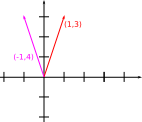
\includegraphics[width = 0.7\linewidth]{2.png}
\end{figure}
\end{minipage}



\begin{minipage}{0.45\textwidth}
\begin{flushleft}
\textit{Dot product is 0}: The vectors are perpendicular to each other. 
\end{flushleft}
\end{minipage} \hfill
\begin{minipage}{0.45\textwidth}
\begin{figure}[H]
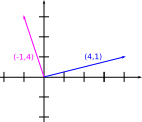
\includegraphics[width = 0.7\linewidth]{3.png}
\end{figure}
\end{minipage}


\begin{minipage}{0.45\textwidth}
\begin{flushleft}
\textit{Negative dot product}: The angle between the vectors is more than $90^\circ$.  
\end{flushleft}
\end{minipage} \hfill
\begin{minipage}{0.45\textwidth}
\begin{figure}[H]
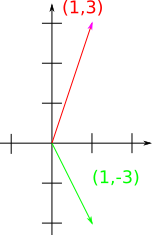
\includegraphics[width = 0.7\linewidth]{4.png}
\end{figure}
\end{minipage}

\

The dot product can even help us find the exact angle between the vectors using the equation in the definition above. 

\paragraph{Example:} "We can use \textbf{this} to calculate \textbf{that}", followed by an example

\paragraph{Mynd?} Always try to have a visual along with the example

\paragraph{Exercise:} Exercise for the reader


		%2.3	Vector dot product 
%
			%What is it/how does it work? 
			%Result is number
			%What does it tell us? 0 = perpendicular


\end{document}